\begin{table}[h]
	\begin{tabular}{|c|c|c|} \hline
	quantity & variable & unit \\ \hline
	traffic density on lane 1 & $\rho_1$ & cars/m \\ \hline
	traffic density on lane 2 & $\rho_2$ & cars/m \\ \hline
	equilibrium velocity on lane 1 & $v_{1e}$ & m/s \\ \hline
	equilibrium velocity on lane 2 & $v_{2e}$ & m/s \\ \hline
	\end{tabular}
	\caption{ variables used in the macroscopic model \label{tab:variables} }
	\end{table}	 
	Traffic flow rate is best captured in a macroscopic model with variables shown in Table \ref{tab:variables}. The total amount of traffic flow will then be determined by
	\begin{align}
	& Q(\rho_1,\rho_2) = \rho_1\cdot v_{1e}(\rho_1,\rho_2)+\rho_2\cdot v_{2e}(\rho_1,\rho_2) & \label{eq:flow}
	\end{align}
	
	We further assume that at equilibrium, there is some velocity-density relation. Given this velocity-density relation, the flow at any given junction of the freeway at a given time is completely determined by the local traffic densities $\rho_1$ and $\rho_2$.
	
	\begin{comment} 
Kerner elt. al. proposed the following relationship in 2002. 
	\begin{align}
	& v_e = v_o\left( (\frac{1+e^{\rho/\rho_m-0.25}}{0.06})^{-1} - 3.76\times10^{-6} \right) & \label{eq:ve}
	\end{align}
	It captures the key 
	\begin{figure}
	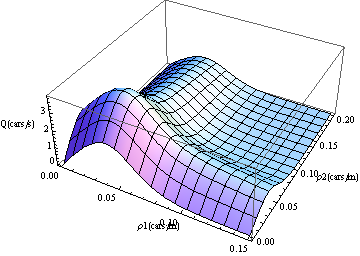
\includegraphics[scale=1]{plot/Q_p1_p2}
	\caption{equilibrium traffic flow as a function of traffic densities using Kerner's velocity-density relation\label{fig:Q_p1_p2}}
	\end{figure}
	\end{comment}
	
	To derive such a relation, we consider all cars to have uniform length $l(m)$, travel with uniform velocity $v_e(\rho)$ and maintain uniform bumper-to-bumper distance $d(m)$ from their neighbors. At this equilibrium, each car will take up a total space of $d+l$ on one lane of the freeway. Since the highway won't be completely conjested all the time, there will normally be extra free space in between cars in addition to the safe following distance. We can think of this free space as being filled by an invisible vihcle density $\rho_0$, therefore
	\begin{align}
	& \rho + \rho_o= \frac{1}{d+l} & \label{eq:follow}
	\end{align}
	Incorporating the two-second rule enforced by the New York Sate Department of Motor Vehicles \cite{science_writing}, $d=v_e(\rho)t$, where $t=2s$. Equation (\ref{eq:follow}) can be solved to obtain and expression for $v_e(\rho)$
	\begin{align}
	& v_e(\rho) =  (\frac{1}{\rho+\rho_o}-l)/t& 
	\end{align}
	We define the capacity (or jamming density) of the road by the density at which traffic stops flowing
	\begin{align}
	& 0 =  (\frac{1}{\rho_j+\rho_o}-l)/t & \\
	\Rightarrow & \rho_j=\frac{1}{l}-\rho_o &
	\end{align}
	This speed-density relationship also imposes a natural speed limit on the road, specifically the speed of traffic at zero density
	\begin{align}
	& v_{nl} = v_e(0) =  (\frac{1}{\rho_o}-l)/t &
	\end{align}
	Consider the natural speed limit of a freeway lane to be $50m/s$, about $110mph$ then $\rho_o=\frac{1}{105}$ and $\rho_j=0.19$
	\begin{figure}[h]
	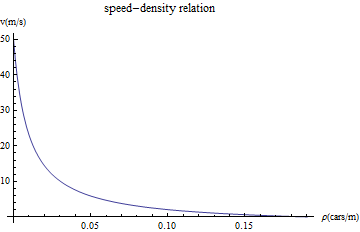
\includegraphics[scale=.6]{plot/speed_density}
	\caption{speed-density relation with a natural speed limit of $50m/s$}
	\end{figure}
	
	With the speed-density relation determined, we can derive the flow of a two-lane freeway using the prescription described in equation \ref{eq:flow}
	\begin{figure}[h]
	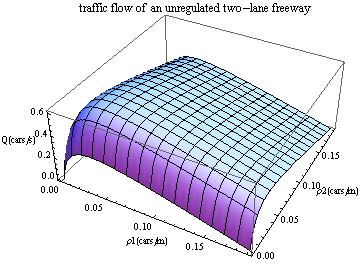
\includegraphics[scale=.6]{plot/unregulated_flow}
	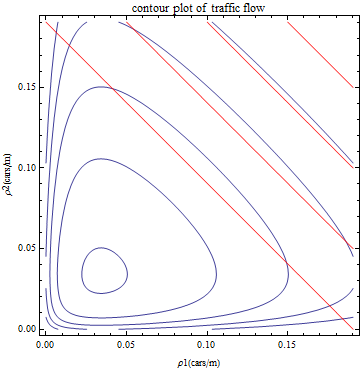
\includegraphics[scale=.45]{plot/contour_flow}
	\caption{traffic flow as a function of lane 1 and lane 2 traffic density on a two-lane freeway}
	\end{figure}
	
	The contour plot provides a good prediction for how the traffic rule might affect the amount of traffic flow. In light traffic, $\rho_1+\rho_2$ is small. As seen in the bottom left corner of the contour plot of traffic flow, any bias in one lane over the other will reduce traffic flow. In this regime, as traffic increase, vehicles should utilize both lanes in the same way to maximize the total amount of traffic flowing through the freeway. However, as traffic satuate the road capacity, bias in the densities of the the roads does not affect traffic flow in a significant manner. This is demonstrated in the contour plot through an overlap of the contour lines of flow(blue) and of total traffic(red) on the road.
	